\documentclass[11pt,a4paper,twocolumn]{article}
\usepackage[utf8]{inputenc}
\usepackage[T1]{fontenc}
\usepackage{amsmath}
\usepackage{amssymb}
\usepackage{amsfonts}
\usepackage{graphicx}
\usepackage[spanish]{babel}
\usepackage{tcolorbox,booktabs,fourier,tabularx,wrapfig,multicol,caption, subcaption,tikz}
\usepackage{import} %Para poder añadir imagenes SVG
%\usepackage{showframe}
\usepackage{tabularx, fancyhdr}
\usepackage[left=2cm,right=2cm,top=2cm,bottom=2cm]{geometry}

\graphicspath{{./ImgMec/}}


\author{Valentin Franzoi}
\title{
\includegraphics[width=.3\textwidth]{utn} \\ \textsc{Mecánica y mecanismos} \\ \textsl{Resumen de fórmulas} \\ }
\date{2022}

%Comando título de cada unidad
\newcommand{\unidad}[2]{\begin{center}
		\fontsize{10}{10}\selectfont\color{gray!50!black}\scshape Unidad #1 \\
		\fontsize{14}{14}\selectfont \scshape #2
		
\end{center}}

\newcommand{\vc}[1]{\textbf{#1}}
\newcommand{\vcs}[1]{\boldsymbol{#1}}
\newcommand{\vcr}[1]{\textbf{\vec{#1}}}
\newcommand{\vcp}[1]{\textbf{\dot{#1}}}
\newcommand{\vcpp}[1]{\textbf{\dot{#1}}}

\fancyfoot[C]{}
\fancyfoot[L]{Valentin Franzoi}
\fancyfoot[R]{\thepage}
\fancyhead[R]{\textsc{Mecánica y mecanismos}}
\renewcommand{\headrulewidth}{0pt}

\begin{document}
	\pagestyle{fancy}
	\maketitle
	\section*{Nomenclatura}
	
	\begin{tabular}{r l}	
%		NADA & \vc{nada}\\
		
	\end{tabular}

	\newpage
	
	\section*{Conceptos}	
	\noindent\textbf{Dinámica}, parte de a mecánica que refiere al análisis de los cuerpos en movimiento. Se divide en :\\
	\textbf{Cinemática:} corresponde al estudio de la geometría del movimiento. Se utiliza para relacionar el desplazamiento, la velocidad, la aceleración y el tiempo, sin hacer referencia a la causa del movimiento.\\
	\textbf{cinética:} estudio de la relación que existe entre las fuerzas que actúan sobre un cuerpo, su masa y el movimiento de este mismo. La cinética se utiliza para predecir el movimiento ocasionado por fuerzas dadas, o para determinar las fuerzas que se requieren para producir un movimiento específico.\\
	
\newpage

	
	\unidad{1}{Cinemática de la partícula}
	Trabajamos con tres casos
	
	\begin{tabular}{r | l} 
		Caso 1& a=f(t) \\ 
		& $dv=a.dt$\\ 
		&$dv=f(t).dt$ \\ 
		& $\int dv=\int f(t).dt$\\ \vspace{.2cm}
		& $dx=v.dt$\\ 
		Cond. iniciales&$\int_{v_{0}}^{v}dv=\int_{0}^{t} f(t).dt$ \\ \vspace{.4cm}
		&$v-v_{0}= \int_{0}^{t} f(t).dt$\\ 
		Caso 2& $a=f(x)$\\ 
		&$v.dv=a.dx$ \\ 
		&$ v.dv=f(x).dx$\\ \vspace{.2cm}
		&$dt=dx/v$\\
		Cond. iniciales& $\int_{v_{0}}^{v}v.dv=\int_{x_{0}}^{c}f(x).dx$\\ \vspace{.4cm}
		& $\frac{1}{2}.v^{2}-\frac{1}{2}.v_{0}^{2}=\int_{x_{0}}^{c}f(x).dx$\\\vspace{.2cm}
		Caso 3& $a=f(v)$\\
		Camino 1& $f(v)=\frac{dv}{dt}$\\
		\vspace{.2cm}
		& $dt=\frac{dv}{f(v)}$\\
		Camino 2&$f(v)=v.\frac{dv}{dx} $\\		\vspace{.4cm}
		&$dx=\frac{v.dv}{f(v)}$\\
		
	\end{tabular}


	\textbf{ Movimiento rectilineo entre particulas}

	\begin{figure}[ht]
		\centering
		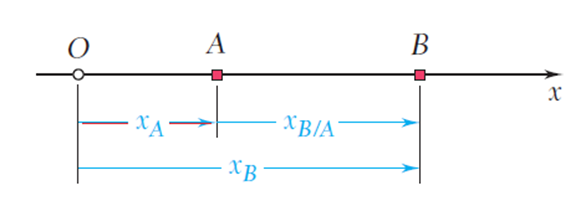
\includegraphics[width=5 cm]{002mec1}
	\end{figure}
	\vspace{-0.4 cm}
	\begin{center}
		$x_{B}=x_{A}+x_{B/A} $\\
		$v_{B}=v_{A}+v_{B/A} $\\
		$a_{B}=a_{A}+a_{B/A} $\\
	\end{center}

	\textbf{Sistemas Coordenados}\\
	Cartesianas:\\
		\begin{figure}[ht]
		\centering
		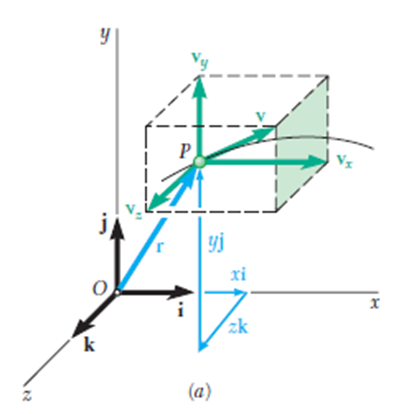
\includegraphics[width=4 cm]{002meccartesianas}
	\end{figure}
		\begin{center}
		$\textbf{r}=x.\textbf{i}+y.\textbf{j}+z.\textbf{k} $\\
		$\textbf{v}=\frac{d\textbf{r}}{dt}=\dot{x}.\textbf{i}+\dot{y}.\textbf{j}+\dot{z}.\textbf{k} $\\
		$\textbf{a}=\frac{d\textbf{v}}{dt}=\ddot{x}.\textbf{i}+\ddot{y}.\textbf{j}+\ddot{z}.\textbf{k} $\\
	\end{center}
\newpage
	Normal y tangencial:\\
	
		\begin{figure}[h]
		\centering
		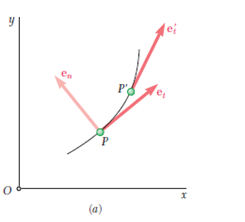
\includegraphics[width=4 cm]{002mecnorytan}
	\end{figure}
	\vspace{-0.4 cm}
	\begin{center}
		\begin{tabular}{r | l} 
			rapidez& $ds/dt=v$\\
			velocidad & $\textbf{v}=v.\textbf{e}_{t}$\\		
			aceleracion& $\textbf{a}=\frac{d\textbf{v}}{dt}=\frac{dv}{dt}.\textbf{e}_{t}+v.\frac{d\textbf{e}_{t}}{dt}$\\
			& $\textbf{a}=\frac{dv}{dt}.\textbf{e}_{t}+\frac{v^{2}}{\rho}.\textbf{e}_{n}$\\
			$a_{tangencial}$&$\frac{dv}{dt}$\\
			$a_{normal}$&$\frac{v^{2}}{\rho}$\\
			Relación $\textbf{e}_{n}-\textbf{e}_{t}$&$\textbf{e}_{n}$=$\frac{d\textbf{e}_{t}}{dt}$\\
		\end{tabular}
	\end{center}

	Normal y tangencial:\\

	\begin{figure}[h]
		\centering
		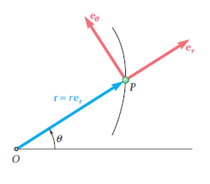
\includegraphics[width=4 cm]{002mecpolar}
	\end{figure}
	\vspace{-0.4 cm}
	\begin{center}
		\begin{tabular}{r | l} 
			velocidad & $\textbf{v}=\dot{r}.\textbf{e}_{r}+r.\dot{\theta}.\textbf{e}_{\theta}$\\		
			aceleracion& $\textbf{a}=(\ddot{r}-r.\dot{\theta}^{2}).\textbf{e}_{r}+(r\ddot{\theta}+2.\dot{r}.\dot{\theta}).\textbf{e}_{\theta}$\\
		\end{tabular}
	\end{center}
	
	\newpage
	
	\unidad{2}{Cuerpo rígido}
	Entendemos por sólido rígido una idealizacion matemática de un sistema físico en la que la distancia entre dos puntos materiales cualesquiera de ellas permanece invariable en el transcurso del tiempo.\\
	\textit{Para cualquier par de puntas A y B del cuerpo, en todo momento} $|\overrightarrow{r}_{B/A}|=cte$\\

	
	\textbf{Tipos de movimiento de un cuerpo rígido:}\\
	
	\textbf{Traslación}\\
	Un movimiento será de traslación si toda línea recta dentro del cuerpo mantiene la misma dirección durante el movimiento. También puede observarse que en la traslación todas las partículas que constituyen el cuerpo se mueven a lo largo de trayectorias paralelas.\\
	En todo momento, todos los puntos del cuerpo tienen la misma \textbf{v} y la misma \textbf{a}.\\
	\begin{center}
		\begin{tabular}{r|l}
		$\overrightarrow{r}_{B/A}$&Módulo Constante\\
		&Dirección Constante\\\vspace{0.4cm}
		&Es un vector Cte en el tiempo\\
		Vectores&$\textbf{r}_{B}=\textbf{r}_{A}+\textbf{r}_{B/A}$\\
		& $\textbf{v}_{B}=\textbf{v}_{A}$\\ \vspace{0.4cm}
		&$\textbf{a}_{B}=\textbf{a}_{A}$\\
	\end{tabular}		
	\end{center}




	\textbf{Rotación alrededor de un eje fijo}\\
	Las particulas que forman el cuerpo rígido se mueven en planos paralelos a lo largo de círculos centrados sobre el mismo eje fijo. Si este eje (eje de rotación) interseca el cuerpo rígido, las partículas localizadas sobre el eje tienen \textbf{v}=0 y \textbf{a}=0.
	
	\begin{center}
		$\vc{v}=\frac{d\vc{r}}{dt}=\vcs{\omega} \times \vc{r}$\\
		$\vc{a}=\vcs{\alpha} \times\vc{r}+\vcs{\omega}\times(\vcs{\omega}\times \vc{r})$
	\end{center}

	Conviene en estos casos trabajar situando el eje Z, perpendicular al la hoja de trabajo para simplificar los calculos vectoriales
	
	\begin{figure}[ht]
		\centering
		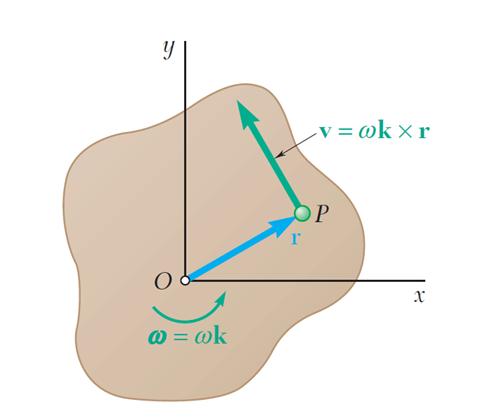
\includegraphics[width=4 cm]{003mecejefijo}
	\end{figure}
	\vspace{-0.7 cm}
	\begin{center}
		$\vc{v}=\vcs{\omega}\vc{k}\times \vc{r}$\\
		$\vc{a}=\vcs{\alpha}\vc{k}\times\vc{r}-\vcs{\omega}^{2}\vc{r}$
	\end{center}

	\newpage
	
	\textbf{Movimiento plano}
	movimientos en los cuales todas las partículas del cuerpo se mueven en planos paralelos. Cualquier movimiento plano que no es ni una rotación ni una traslación se conoce como un movimiento plano general.
	
	\begin{figure}[ht]
		\centering
		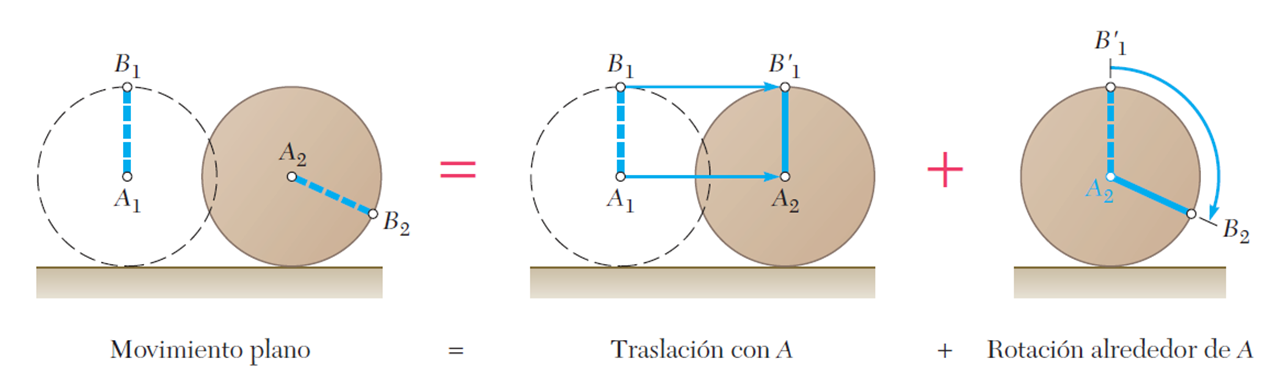
\includegraphics[width=8 cm]{003mecmovplano}
	\end{figure}

	\noindent Los vectores $\vcs{\alpha}$ y $\vcs{\omega}$ son perpendiculares al plano de movimiento.\\
	Los vectores \vc{v} y \vc{a} de cada punto del cuerpo están contenidos en el mismo plano 
	
	\begin{figure}[ht]
		\centering
		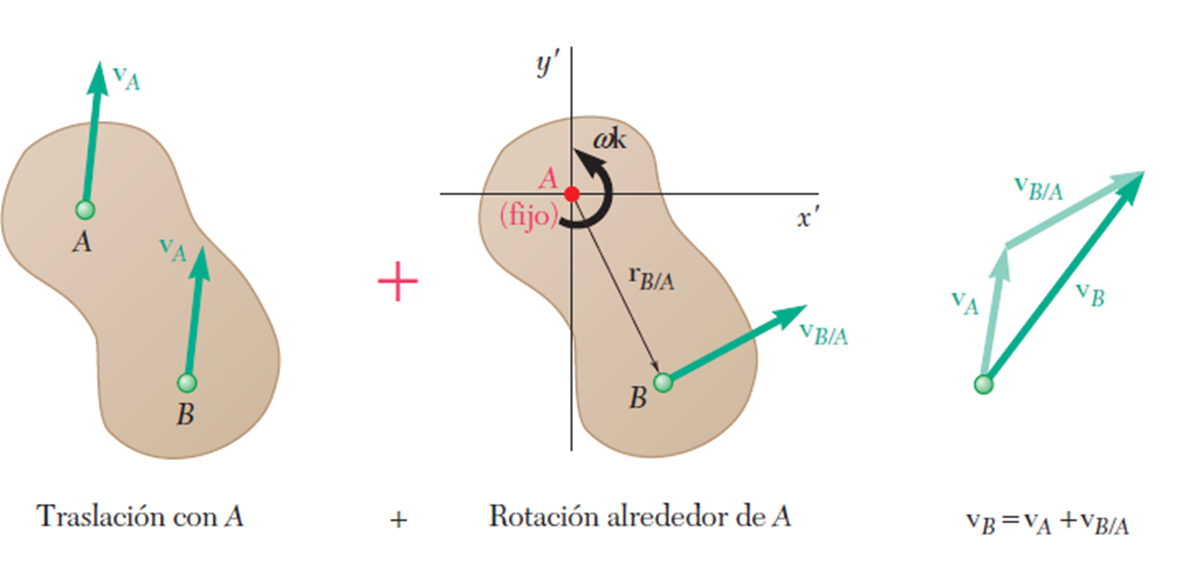
\includegraphics[width=8 cm]{003mecmovplano2}
	\end{figure}
	
	Las velocidades en el movimiento plano son:
	\begin{center}
		 $\vc{v}_{B}=\vc{v}_{A}+\vc{v}_{B/A}$\\
		 $\vc{v}_{B/A}=\vcs{\omega}\vc{k}\times\vc{r}_{B/A}$\\
		 $\vc{v}_{B}=\vc{v}_{A}+\vcs{\omega}\vc{k}\times\vc{r}_{B/A}$\\
	\end{center}

	\textbf{Traslación}\\
	Se afirma que un movimiento será de traslación si toda línea recta dentro del cuerpo mantiene la misma dirección durante el movimiento. Se observa que en la traslaci+on todas las particulas que constituyen el cuerpo se mueven a lo largo de trayectorias paralelas.\\
	\begin{figure}[ht]
		\centering
		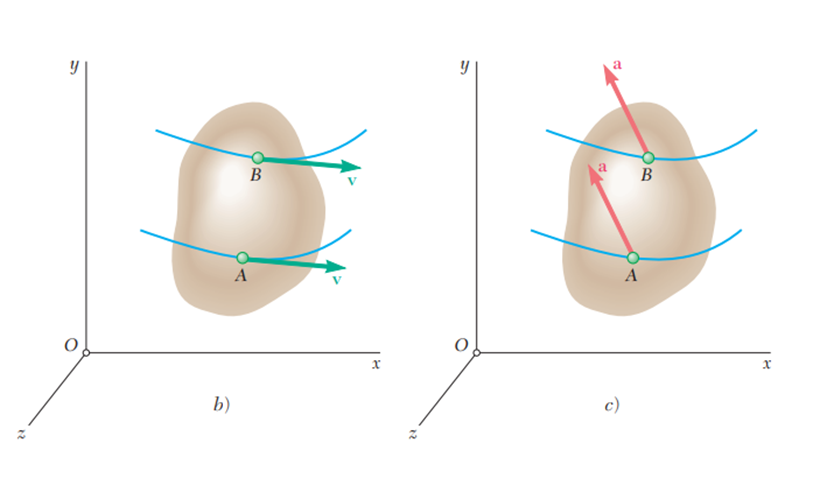
\includegraphics[width=8 cm]{003traslacion}
	\end{figure}
		\begin{center}
		$\vc{v}_{B}=\vc{v}_{A}$\\
		$\vc{a}_{B}=\vc{a}_{A}$\\
	\end{center}

	\textbf{Rotación alrededor de un eje fijo}\\
	En este movimiento las partículas que forman el cuerpo rígido se mueven en planos paralelos a lo largo de círculos centrados sobre el mismo eje fijo.\\
	\begin{figure}[ht]
		\centering
		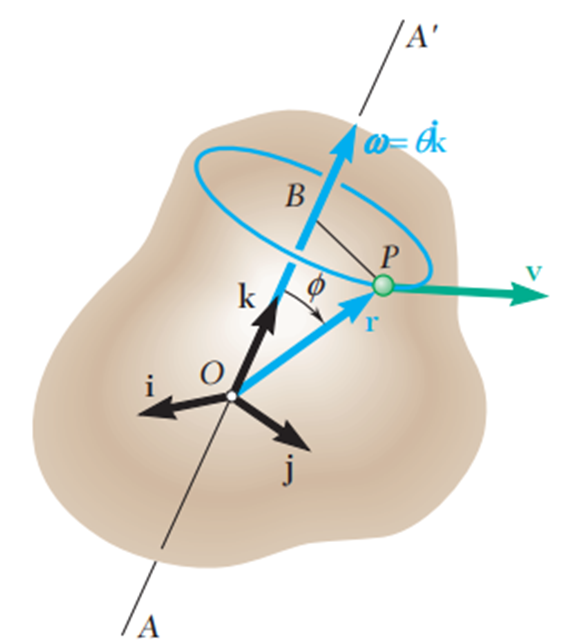
\includegraphics[width=4 cm]{003rotejefijo}
	\end{figure}

	\begin{center}
		$\vc{v}=\vcs{\omega}\times\vc{r}$\\
		$\vc{a}=\vcs{\alpha}\times\vc{r}+\vcs{\omega}\times(\vcs{\omega}\times\vc{r})$\\
	\end{center}

	\noindent Trabajando en el plano, haciendo coincidir el $\vec{\vc{k}}$, con el eje de nuestro sistema de referencia queda:
	\begin{center}
	$\vc{v}=\omega\vec{\vc{k}}\times\vc{r}$\\
	$\vc{a}=\alpha\vec{\vc{k}}\times\vc{r}-\omega^{2}\vc{r}$\\	
	\end{center}	

	\textbf{Movimiento plano}\\
	Nosotros tratamos los movimientos planos en los cuales todas las particulas del cuerpo se mueven en planos paralelos.\\
	Velocidades en el mov. plano:

	\begin{center}
		$\vc{v}_{b}=\vc{v}_{a} + \vc{v}_{b/a}$\\
		$\vc{v}_{b}=\vc{v}_{a}+\omega\vec{\vc{k}}\times\vc{r}_{b/a}$

	\end{center}

	\textbf{Centro instantáneo de Rotación}\\
	Considere el movmimiento plano general de una placa, en cualquier instante dado de la velocidad de las diversas partículas de la placa es la misma como si la placa girara alrededor de cierto eje perpendicular a su plano.\\
	\begin{figure}[ht]
		\centering
		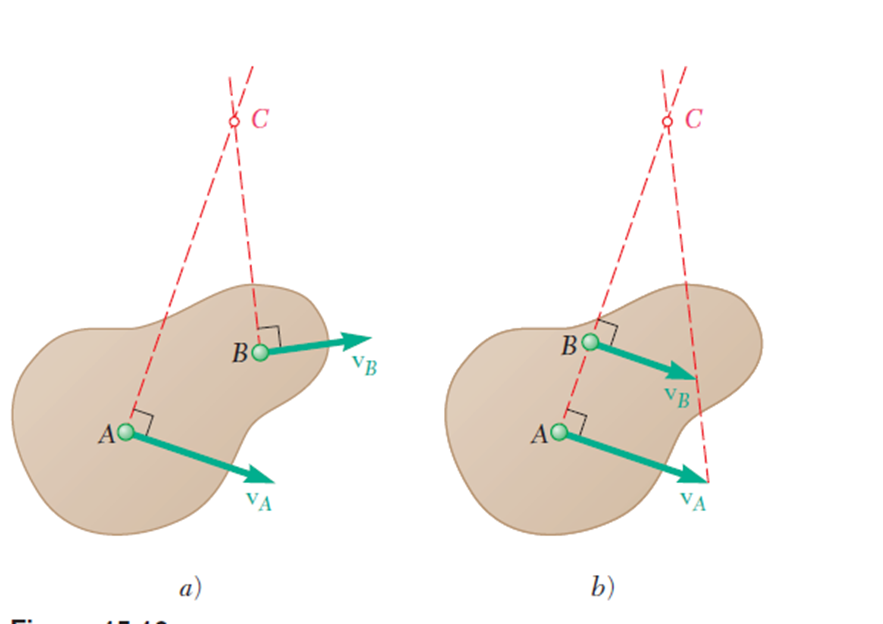
\includegraphics[width=8 cm]{003cir}
	\end{figure}


	\textbf{Movimiento respecto a un sistema de referencia en rotación}\\
	\begin{center}
		$\vc{v}_{xy}=\vc{v}_{x'y'} + \Omega \times \vc{r}$\\
	\end{center}

	\begin{table}[!htbp]
		\centering
		\begin{tabularx}{0.5\textwidth}{rX}
			$\vc{v}_{xy}$& Velocidad absoluta del punto\\
			$\vc{v}_{x'y'}$& Velocidad del unto relativa al sistema de referencia en rotación\\
			$\Omega$ & Velocidad angular del sistema móvil respecto del fijo\\
			$\vc{r}$ &Posición del punto en el sistema móvil\\
%			&\\
		\end{tabularx}
	\end{table}
	
	\begin{center}
		$\vc{a}_{xy}=\vc{a}_{x'y'} + \dot{\Omega} \times \vc{r}+ \Omega \times (\Omega \times \vc{r}) + 2 (\Omega \times (\vc{v}_{x'y'}))$\\
	\end{center}
	
	\begin{table}[!htbp]
		\centering
		\begin{tabularx}{0.5\textwidth}{rX}
			$\vc{a}_{xy}$&Aceleración absoluta del punto\\
			$\vc{a}_{x'y'}$&Aceleración relativa al sistema de referencia móvil\\
			$\dot{\Omega}$&Aceleración angular del sistema móvil respecto del sistema fijo\\
			$\Omega$& Velocidad angular del sistema móvil respecto del sistema fijo\\
			$\vc{r}$& posición de la partícula representada en el sistema de referencia móvil\\
			$\vc{v}_{x'y'}$&Velocidad respecto del sistema móvil\\
			$2 (\Omega \times (\vc{v}_{x'y'}))$&Aceleración de Coriolis.\\
%			&\\
		\end{tabularx}%
	\end{table}%

	\textbf{Rotación alrededor de un punto fijo}\\
	Teorema de Euler: \textit{``Cuando un sólido rígido gira alrededor de un punto fijo, toda posición del sólido se puede obtener a partir de cualquier otra posición mediante una sola rotación en torno a un cierto eje que pasa por dicho punto fijo''}, es decir, dos rotaciones ``componentes'' alrededor de ejes diferentes que pasan por un punto equivalen a una sola rotación resultante alrededor de un eje que pasa por el punto.

\newpage	
	\unidad{4}{Dinámica de la particula}
%	La dinámica de la partícula se puuede estudiar desde tres enfoques:
%	\begin{tabular}{r l}
%		Leyes de Newton & $\sum \vc{F}= m \vc{a}$\\
%		Trabajo y energía & $U_{1\rightarrow2} = T_{2} - T_{1}$\\
%							& $T= \frac{1}{2} mv^{2}$\\
%							& $U_{1\rightarrow2}=\int_{1}^{2} \vc{F}.d\vc{r}$\\
%		Cantidad de movimiento &$m\vc{v}_{1}+\int_{t1}^{t2} \vc{F}.dt=m\vc{v}_{2}$\\
%							&$\sum m\vc{v}_{1}+\sum \vc{F}\Delta t = \sum m \vc{v}_{2}$\\
%							&$ m\vc{v}_{1}+\vc{Imp}_{1\rightarrow2} =m \vc{v}_{2}$\\
%	\end{tabular}
%	
	\begin{tcolorbox}
		\begin{tabular}{ c c }
			\textbf{Leyes de Newton} & 	\textbf{Cantidad de movimiento}\\
			\begin{tabular}{r l}
				1° & $\sum \vc{F}_{r}=0$\\
				2° & $\sum \vc{F}_{r}=\vc{m}\vc{a}$\\
				3° & $\vc{F}_{12}=-\vc{F}_{21}$\\
			\end{tabular}
			&
			\begin{tabular}{r l}
				Lineal & $\vc{L}=m\vc{V}$ \\
				Angular & $\vc{H}_{o}= \vc{r}\times m.\vc{v}$\\
			\end{tabular}\\
		\end{tabular}\\	
	\end{tcolorbox}
	


	\textbf{Energía cinetica de una particula, principio del trabajo y la energía}
	\begin{center}
		$U_{1\rightarrow2}=T_{2}-T_{1}$
	\end{center}
	\begin{tabular}{r l}
	$U_{1\rightarrow2}$ & Trabajo realizado  \\
	$T$ & Energía cinética\\
	\end{tabular}\\

	''Energía cinética de una partícula representa también la capacidad para realizar trabajo asociado con la velocidad de la partícula´´\\
	
	\textbf{Potencia y eficiencia}\\
	\begin{tcolorbox}
		\begin{tabular}{r l}
			Potencia & $\frac{dU}{dt}=\frac{\textbf{F}.\textbf{dr}}{dt}=\vc{F}.\vc{v}$\\
			Rendimiento & $\eta	=\frac{potencia~de~salida}{potencia~de~entrada}$\\
		\end{tabular}\\
	\end{tcolorbox}
	
	\textbf{Energía potencial y fuerzas conservativas}\\
	Cuando el trabajo realizado por una fuerza no depende de la trayectoria de la partícula hablamos de una fuerza conservativa.
		\begin{center}
		$U_{1\rightarrow2}=V_{1}-V_{2} = -\Delta V$
	\end{center}
	\begin{tabular}{r l}
		$U_{1\rightarrow2}$ & Trabajo realizado  \\
		$V$ & Energía potencial\\
	\end{tabular}\\

	\textbf{Energía mecánica}\\
	Conociendo que:\\
	\begin{tabular}{r l}
		$U_{1\rightarrow2}=$&$V_{1}-V_{2}$\\
		$U_{1\rightarrow2}=$&$T_{2}-T_{1}$\\
	\end{tabular}

	Igualando nos queda $V_{1}+T_{1}=V_{2}+T_{2}$, a la suma de $T+V$ le llamaremos $E_{m}$ (Energía Mecánica).\\
	\begin{tcolorbox}
	Si todas las $\vc{F}$ que actúan sobre una partícula son conservativas $E_{m}=$ CTE. = $T_{n}+V_{n}$\\
	Si sobre la partícula actúan $\vc{F}$ no conservativas	$U_{1\rightarrow2~F~no~cons}=\Delta E_{m}$.
	\end{tcolorbox}
	
	\textbf{Impulso y cantidad de movimiento}\\
	\begin{tabular}{r l}
		$\vc{F}=\frac{d}{dt}(m\vc{v})$&$\int_{t_{1}}^{t_{2}} \vc{F}.dt= m \vc{v}_{2} - m \vc{v}_{1}$\\
		&$m \vc{v}_{1}+\int_{t_{1}}^{t_{2}} \vc{F}.dt= m \vc{v}_{2}$\\
		$\vc{F}$& son las fuerzas impulsivas\\
	\end{tabular}

	Esto te arma un sistema de tres ecuaciones:\\
	\begin{tcolorbox}	
		\begin{tabular}{l}
			$(m\vc{v}_{x})_{1}+\int_{t1}^{t2} \vc{F}_{x} dt=(m\vc{v}_{x})_{2}$\\
			$(m\vc{v}_{y})_{1}+\int_{t1}^{t2} \vc{F}_{y} dt=(m\vc{v}_{y})_{2}$\\
			$(m\vc{v}_{z})_{1}+\int_{t1}^{t2} \vc{F}_{z} dt=(m\vc{v}_{z})_{2}$\\
		\end{tabular}
	\end{tcolorbox}

	\unidad{4}{Sistema de partículas}
	\textbf{Aplicación de las leyes de Newton al movimiento de un sistema de partículas. Fuerzas efectivas.}\\
	Sobre cada particula actúan fuerzas internas y externas:
	\begin{center}
			$\vc{F}_{i}+\sum_{j=1}^{n} \vc{f}_{ij}=m_{i}\vc{a}_{i}$\\
			\vspace{0.2cm}
			$\vc{r}_{i}\times\vc{F}_{i}+\sum_{j=1}^{n}(\vc{r}_{i}\times \vc{f}_{ij})=\vc{r}_{i}\times m_{i}\vc{a}_{i}$\\		
	\end{center}
	
	 pero se demuestra que las internas se cancelan entre sí:
	 \begin{center}
	 	$\sum_{j=1}^{n} \vc{f}_{ij}=0$\\
	 	\vspace{0.2cm}
	 	$\sum_{j=1}^{n}(\vc{r}_{i}\times \vc{f}_{ij})=0$\\		
	 \end{center}
	
	Nos queda:
	\begin{tcolorbox}
	\begin{center}
		$\sum_{j=1}^{n}\vc{F}_{i}=\sum_{j=1}^{n} m_{i}\vc{a}_{i}$\\
		\vspace{0.2cm}
		$\sum_{j=1}^{n}(\vc{r}_{i}\times\vc{F}_{i})=\sum_{j=1}^{n}(\vc{r}_{i}\times m_{i}\vc{a}_{i})$\\		
	\end{center}	
	\end{tcolorbox}

	Si derivamos el vector cantidad de movimiento lineal y el vector cantidad de movimiento angular alrededor de O respecto del tiempo, obtenemos :\\
	
	\begin{tcolorbox}
		\begin{center}
			\begin{tabular}{ r c l }
				$\sum \vc{F}= $&$\dot{\vc{L}}=$&$ \sum_{i=1}^{n}m_{i}\vc{a}_{i}$\\
				$\sum \vc{M}_{o}= $&$\dot{\vc{H}}_{o}=$&$ \sum_{i=1}^{n}(\vc{r}_{i}\times m_{i}\vc{a}_{i})$
			\end{tabular}
		\end{center}
	\end{tcolorbox}
	
	\textbf{Centro de masa}
	\vspace{-0.55cm}
	\begin{center}
		\begin{tabular}{ r c l }
			&$m\bar{\vc{r}}=\sum_{i=1}^{n} m_{i}\vc{r}_{i} $& \\
			$m\bar{x}=\sum_{i=1}^{n} m_{i}x_{i}$&$m\bar{y}=\sum_{i=1}^{n} m_{i}y_{i}$ &$m\bar{z}=\sum_{i=1}^{n} m_{i}z_{i}$ \\
		\end{tabular}
	\end{center}
	Diferenciando respecto a \textit{t} obtenemos:
	\begin{center}
		\begin{tabular}{ r l }
			$m\dot{\bar{\vc{r}}}=\sum_{i=1}^{n} m_{i}\dot{\vc{r}_{i}} $&$m\bar{\vc{v}}=\sum_{i=1}^{n} m_{i}\vc{v}_{i} $\\
		\end{tabular}
	\end{center}

	\begin{tcolorbox}
			\begin{center}
			\begin{tabular}{ r l }
				$\vc{L}=m\bar{\vc{v}} $&$\dot{\vc{L}}=m\bar{\vc{a}}$\\
			\end{tabular}\\
			$\sum\vc{F}=m\bar{\vc{a}}$
		\end{center}
	\end{tcolorbox}

	\textbf{Cantidad de movimiento angular de un sistema de partículas alrededor de su centro de masa}\\
	se trabaja con dos sistemas de referencia, absoluto ($O_{xyz}$) y ($G_{x'y'z'}$).\\
	 \textit{El momento resultante alrededor de G de las fuerzas externas es igual a la razón de cambio de la cantidad de movimiento angular alrededor de G del sistema de partículas.}\\
	
	\begin{tcolorbox}
		\begin{center}
			$ \sum \vc{M}_{G}=\dot{\vc{H}}'_{G} = \dot{\vc{H}}_{G}$\\
			$\vc{H}_{G}=\sum_{i=1}^{n}(\vc{r}'_{i}\times m_{i}\vc{v}_{i})=\sum_{i=1}^{n}(\vc{r}'_{i}\times m_{i}\vc{v}'_{i})$
		\end{center}
	\end{tcolorbox}

	\textbf{Energía cinética de un sistema de partículas}\\
	Haciendo uso de un sistema de referencia centroidal, sistemas de referencia ($O_{xyz}$) y ($G_{x'y'z'}$)\\
	La energía cinética T de un sistema de partículas puede obtenerse al sumar la energía cinética del centro de masa G (suponiendo que toda la masa está concentrada en G) y la energía cinética del sistema en su movimiento relativo al sistema de referencia ($G_{x'y'z'}$)
	\begin{tcolorbox}
		\begin{center}
			$\vc{T}=\frac{1}{2} m \bar{v}^{2} +\frac{1}{2}'\sum_{i=1}^{n}m_{i} v'^{2}_{i}$\\
		\end{center}
	\end{tcolorbox}	
	
	El principio de energía y trabajo puede aplicarse, la cantidad $U_{1~\rightarrow~2}$ representa el trabajo de todas las fuerzas que actúan sobre las partículas del sistema, se debe considerar el trabajo de las fuerzas internas y externas.\\
	Si todas las fuerzas que actúan sobre las partículas del sistema son conservativas, se puede aplicar principio de conservación de la energía.\\
	\begin{tcolorbox}
		\begin{center}
			$T_{1}+U_{1~\rightarrow~2}=T_{2}$\\
			$T_{1}+V_{1}=T_{2}+V_{2}$\\
		\end{center}
	\end{tcolorbox}	
	
	\textbf{Impulso y cantidad de movimiento de un sistema de partículas}\\
	Se hacen presentes impulsos lineales y angulares\\
	\begin{tcolorbox}
		\begin{center}
			$\vc{L}_{1}+\sum \int_{t_{1}}^{t_{2}} \vc{F} dt=\vc{L}_{2}$\\
			$(\vc{H}_{O})_{1}+ \sum \int_{t_{1}}^{t_{2}} \vc{M}_{O} dt=(\vc{H}_{O})_{2} $\\
		\end{center}
	\end{tcolorbox}	
	
	
	\textbf{Sistemas variables de partículas.\\
		 Corriente estacionaria de partículas}\\
	\textit{El sistema formado por la cantidad de movimiento} $()\Delta m) \vc{v}_{A}$ \textit{de las partículas que entran a} S \textit{en el tiempo } $\Delta t$ \textit{y los impulsos de las fuerzas ejercidas sobre} S \textit{durante ese tiempo es equipolente a la cantidad de movimiento} $(\Delta m) \vc{v}_{B}$ \textit{de las partículas que salen de} S \textit{en el mismo tiempo} $\Delta t$\\

	\begin{center}
		$(\Delta m) \vc{v}_{A}+\sum \vc{F} (\Delta t) =(\Delta m) \vc{v}_{B}$\\
		\vspace{0.3cm}
		$\sum \vc{F} =\dfrac{dm}{dt} (\vc{v}_{B}-\vc{v}_{A})$\\
	\end{center}

	\unidad{5}{Dinámica del cuerpo rígido en movimiento plano}
	\textbf{Cinetica de cuerpos rígidos}
	\begin{center}
	$ {\vc{H}}_{G}=\bar{I}\vcs{\omega} \rightarrow  \dot{\vc{H}}_{G}=\bar{I}\vcs{\dot{\omega}}=\bar{I}\vcs{\alpha}$
	\end{center}

	\begin{tcolorbox}
		\begin{center}
			\begin{tabular}{c c c}
				$\sum F_{x}=m\bar{a_{x}} $&$\sum F_{y}=m\bar{a_{y}} $ & $\sum M_{G}=\bar{I}\alpha$\\
			\end{tabular}
		\end{center}
	\end{tcolorbox}
	Principio de d'Alembert: las fuerzas externas que actúan sobre un cuerpo rígido son realmente \textbf{equivalentes} a las fuerzas efectivas de las diversas partículas que forman el cuerpo
	\begin{center}
		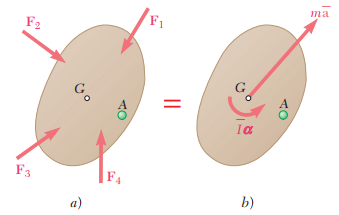
\includegraphics[width=6cm]{dalembert}
	\end{center}
	Si se presenta una \textbf{rotación no centroidal}, desarrollando queda:
	\begin{center}
		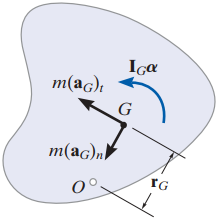
\includegraphics[width=3cm]{CRrotnocen}\\
		$ \sum M_{O}=\bar{I}\vcs{\alpha}+(m.\bar{a})_{t}).\bar{r}$ siendo $ \bar{r}\vcs{\alpha}=\bar{a}$\\
		$M_{O}=\bar{I}\vcs{\alpha}+(m.\bar{r}\vcs{\alpha}).\bar{r}$\\
		$M_{O}=(\bar{I}+m.\bar{r}^{2}).\vcs{\alpha}$
		\begin{tcolorbox}
			\begin{center}
				$\sum M_{O}=I_{O}\vcs{\alpha}$
			\end{center}
		\end{tcolorbox}
	\end{center}
\textbf{Energía y cantidad de movimiento de cuerpos rígidos}\\
Particularmente útil para resolver problemas que implican miembros conectados por pasadores, bloques y poleas que se conectan mediante cuerdas inextensibles y engranajes dentados. En todos estos casos las fuerzas internas se presentan por pares de fuerzas iguales y opuestas, los puntos de aplicación de las fuerzas se mueven distancias iguales durante un pequeño desplazamiento del sistema. Como resultado, el trabajo de las fuerzas internas es cero, y $\vcs{U_{1\rightarrow2}}$ se reduce al trabajo de las fuerzas externas al sistema.\\


\textbf{Impulso y cantidad de movimiento p. movimiento plano de un cuerpo rígido}\\

\end{document}